
\documentclass[a4paper,10pt]{article}

\usepackage{geometry}

\usepackage[utf8x]{inputenc}
\usepackage[bookmarks,colorlinks=false,pdfborder={0 0 0}]{hyperref}
\hypersetup{pdftitle={2. Praktikum: Technik und Technologie}}
\usepackage{url}
\usepackage[ngerman]{babel}
\usepackage{graphicx}
\usepackage{listings}

\parindent 0pt 
\parskip 10pt

\title{2. Praktikum: Technik und Technologie}
\author{Andreas Krohn \and Benjamin Vetter}

\begin{document}

\maketitle

\section{Kurzdokumentation}

\section{Erklärung Ihrer Beobachtungen zur Multicast Paketverteilung}

\subsection{Wie erreichen die Multicast Daten Ihren Rechner auf der Ethernet Protokollebene?}

Hierzu werden die Multicast IP Host Group Adressen auf Ethernet Multicast Adressen gemappt,
indem die low-order 23 bit der IP-Adresse auf die low-order 23 bit der Ethernet Multicast Adressen gemappt werden (01-00-5E-00-00-00).
Da viele Ethernet-Netzwerkkarten bzgl. der konfigurierbaren Adressen, für die sie zuständig sein sollen, eingeschränkt sind, muss ggf. der Adress-Filter der Karte ausser Kraft gesetzt werden.
Hierdurch nimmt die Netzwerkkarte alle Pakete entgegen, auch wenn sie gar nicht für das Interface bestimmt sind (vgl. \url{http://tools.ietf.org/html/rfc1112}).

\subsection{Welchen Einfluss hat Ihr IGMP join?}

Der IGMP Join selbst hat keinen Einfluss auf das Verhalten auf Ethernet-Ebene,
da wir bspw. mithilfe des Sniffers beobachten konnten, 
dass auch nach einem IGMP Leave weiterhin die Multicast-Pakete den Host erreicht haben,
wenngleich diese auch nicht bis zur Anwendungsebene hochgereicht wurden (vgl. Abbildrung \ref{multicast_after_leave}).

\begin{figure}
	\begin{center}
		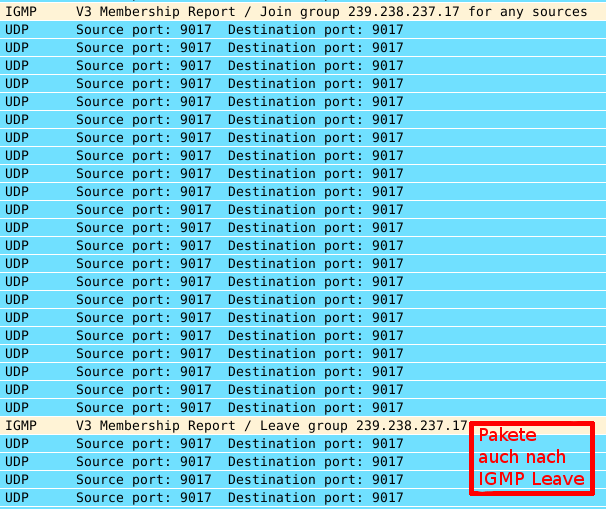
\includegraphics[width=0.5\textwidth]{multicast_after_leave.png}
	\end{center}

	\caption{IGMP Join/Leave bzgl. Ethernet-Ebene}

	\label{multicast_after_leave}
\end{figure}

Insofern hat das IGMP Join nur Auswirkungen auf den Stack des Hosts, 
der die IGMP-Join Nachricht abgesetzt hat.

\end{document}


